\label{appendix:guia}
%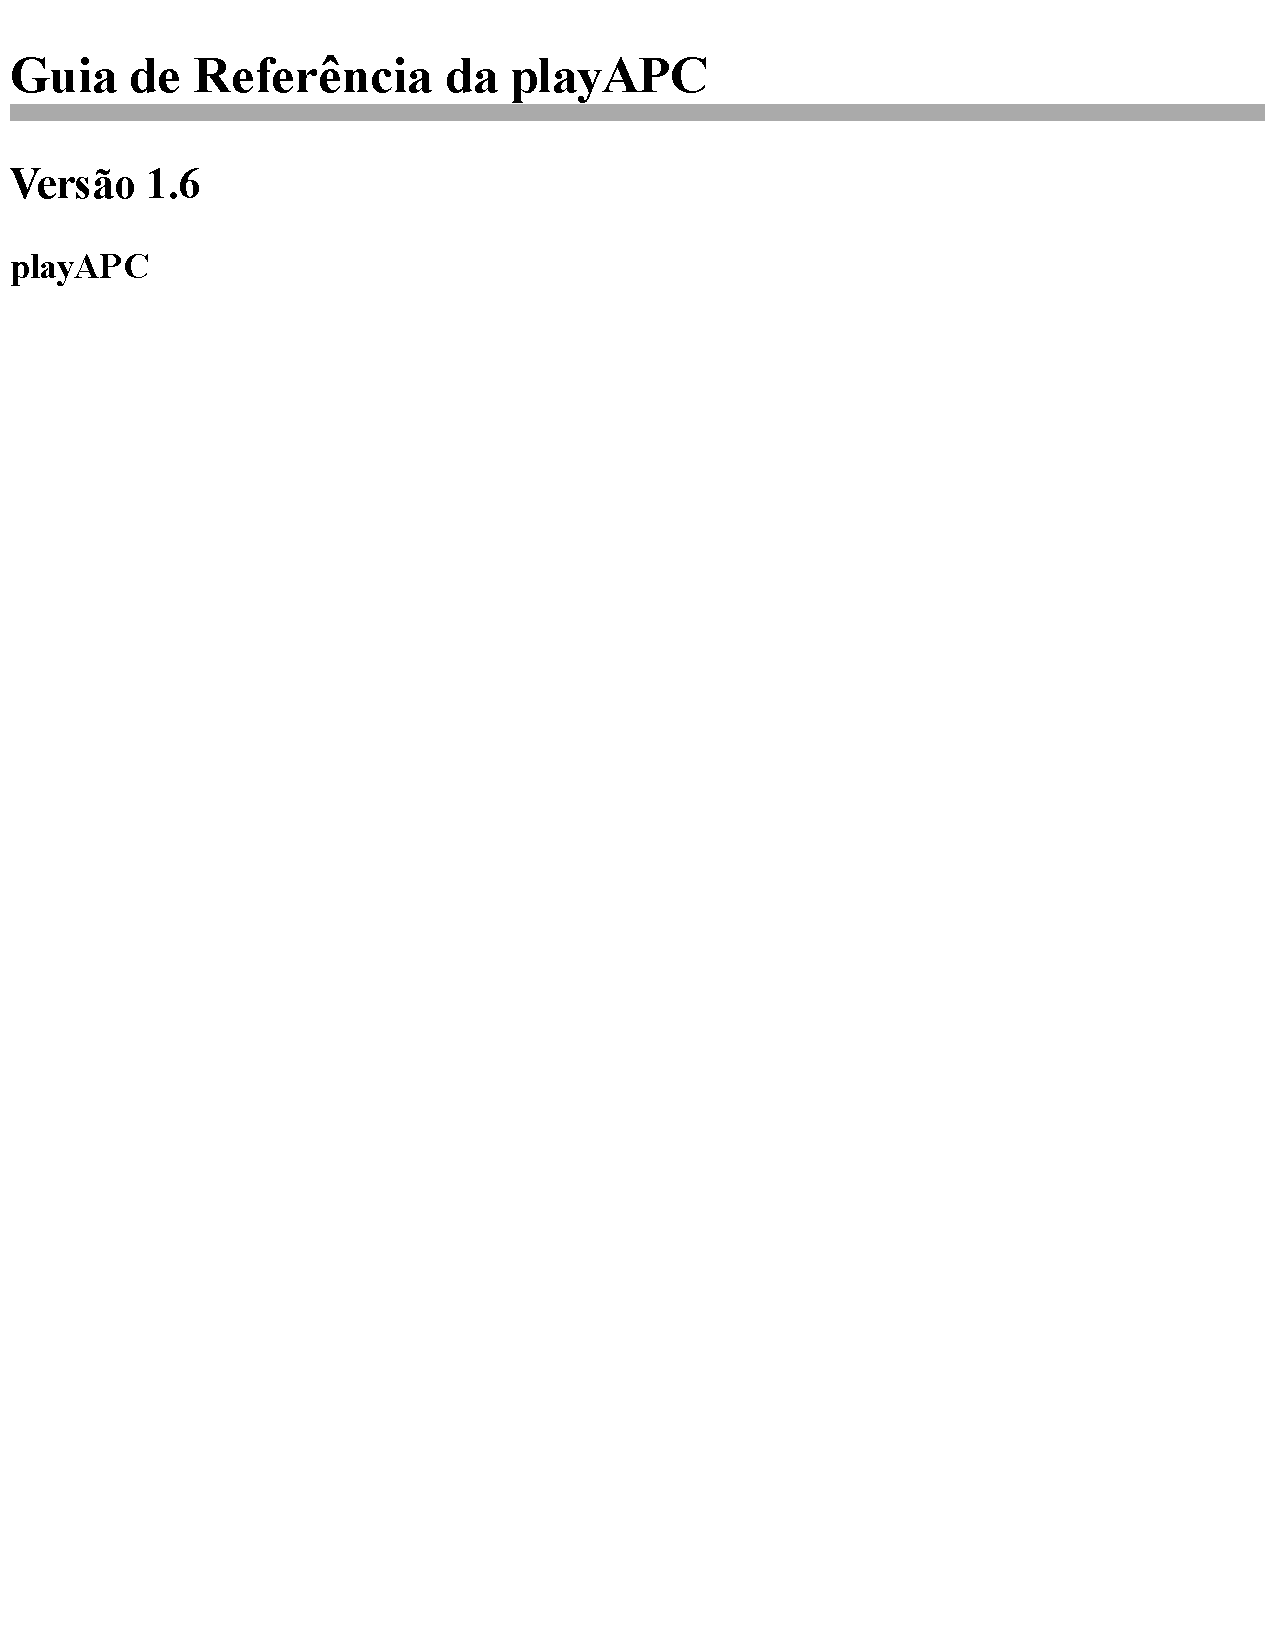
\includepdf[pages={1-}]{apendice/guia.pdf}

\figura[!h]{../img/guia.png}{Tela principal do Guia de Referência}{fig:guia}{width=1.0\textwidth}%
\newpage

O Guia de Referência, disponibilizado em plataforma online, está separado em quatro guias de navegação:
\begin{enumerate}
	\item Instalação
	\item Documentação
	\item Lista de Funções
	\item Exemplos
\end{enumerate}

\section{Instalação}

O Guia ilustra passo a passo o processo de instalação da biblioteca, separado por sistema operacional. Há a aba para Windows, Linux e Mac. Para os três sistemas operacionais, há pelo menos quatro seções para o processo de instalação:
\begin{enumerate}
	\item Verificação se o computador tem suporte à OpenGL
	\item Instalação de dependência 
	\item Instalação dos binários da biblioteca
	\item Verificação de a biblioteca foi corretamente instalada 
\end{enumerate}
Para o sistema operacional Windows, há ainda um vídeo-tutorial explicando como realizar a instalação da biblioteca, englobando os passos de instalação de dependências até a verificação se foi instalada corretamente.

\section{Documentação}

O Guia de Referência apresenta a documentação das funções da interface da \playAPC{}, assim como está indicado na Seção \ref{sec:requisitos}. Detalhes de implementação não foram descritos por não ser interessante no ponto de vista do aluno, o qual apenas precisa saber como utilizar as funções. Cada função documentada apresenta um resumo da sua ação e uma explicação de seus argumentos e retorno quando existirem. Além disso, cada função possui, pelo menos, um exemplo de como utilizá-la, com capturas de tela e código fonte. 

\section{Lista de funções}

O Guia disponibiliza uma navegação rápida para busca de funções, listando todas as funções criadas em ordem alfabética e listando-as também por versões da biblioteca.

\section{Exemplos}
O Guia disponibiliza cinco exemplos criados pelos desenvolvedores da biblioteca, mostrando como utilizar um conjunto diferenciado de funções da \playAPC{} em programas mais contextualizados.
Há ainda uma aba de exemplos criados pelos alunos que utilizaram a biblioteca, sendo disponibilizado apenas os executáveis de seus programas. Os programas atualmente disponíveis foram cedidos pelos alunos das turmas E e H do semestre 2/2016 ,  ministrado pelos professores Alexandre Zaghetto e Carla Castanho.